\chapter{Appendix}\label{cha::appendix}
	\section{Quantitative Analysis}
	\subsection{Landmark Registration Error (LRE)}	
	\begin{figure}[h]
		\centering
		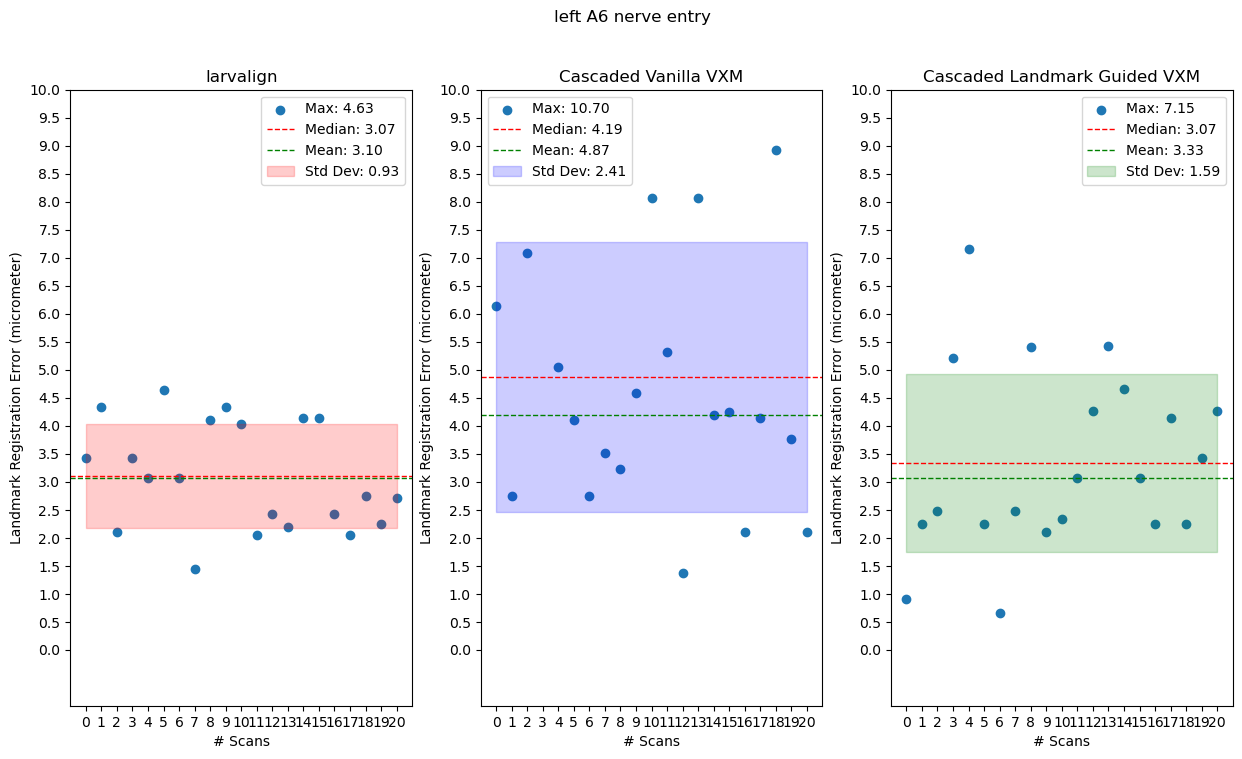
\includegraphics[width=0.75\columnwidth]{resources/chapter5_fresh/output/left A6 nerve entry.png}
		\caption{LRE plot distribution for "left A6 nerve entry" landmark point measured across different scans from the "medium" quality \texttt{Larvalign dataset}.}
		\label{fig:landmark1}
	\end{figure}

	\begin{figure}[h]
		\centering
		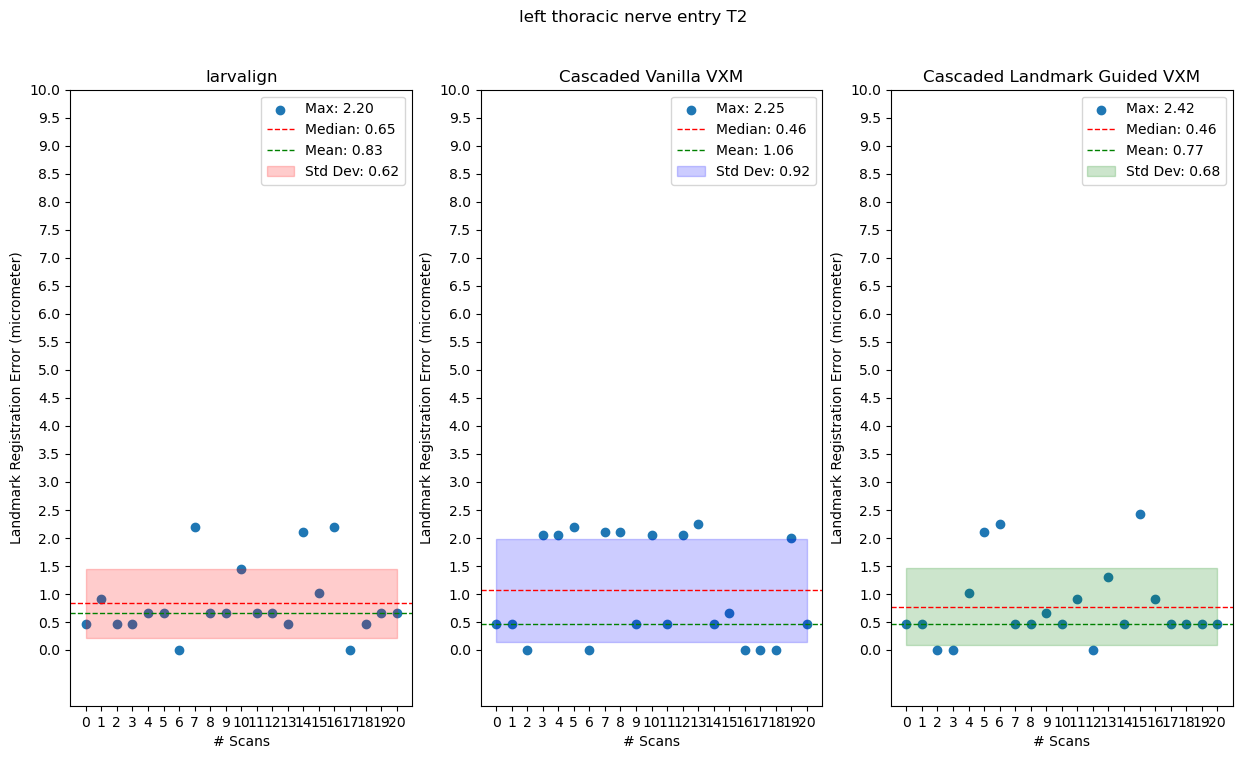
\includegraphics[width=0.75\columnwidth]{resources/chapter5_fresh/output/left thoracic nerve entry T2.png}
		\caption{LRE plot distribution for "left thoracic nerve entry T2" landmark point measured across different scans from the "medium" quality \texttt{Larvalign dataset}.}
		\label{fig:landmark2}
	\end{figure}

	\begin{figure}[h]
		\centering
		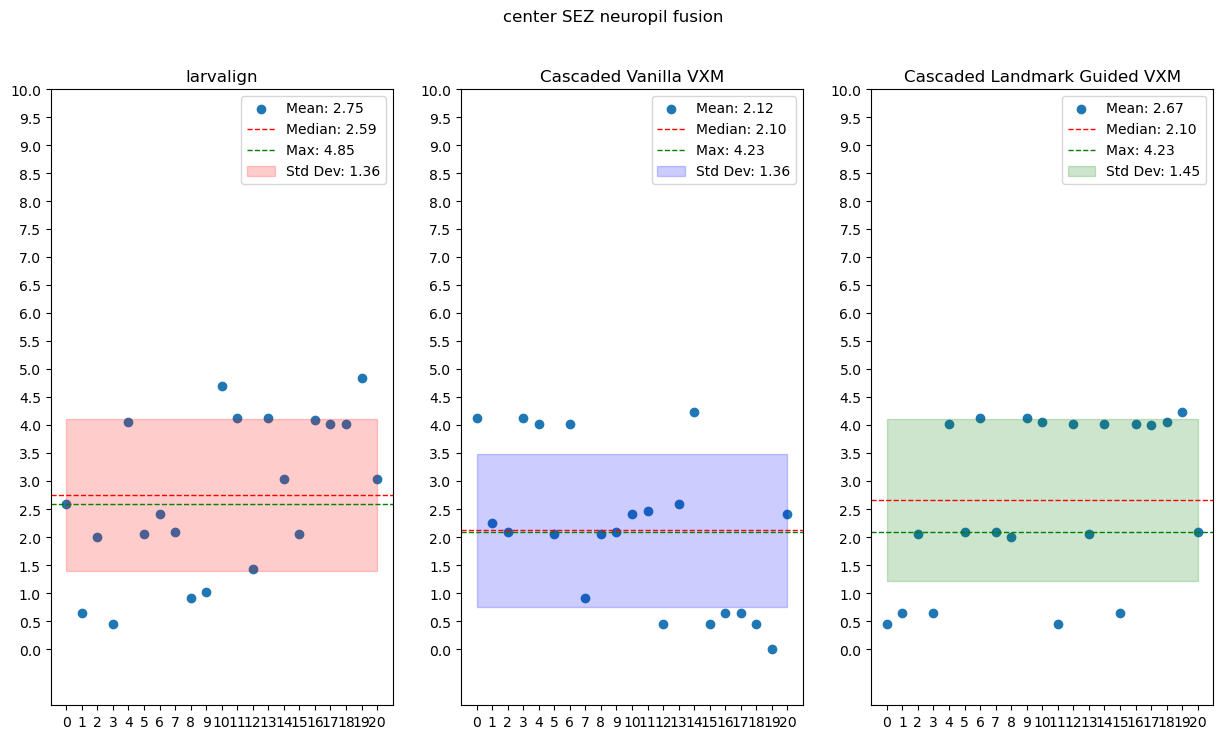
\includegraphics[width=0.75\columnwidth]{resources/chapter5_fresh/output/center SEZ neuropil fusion.png}
		\caption{LRE plot distribution for "center SEZ neuropil fusion" landmark point measured across different scans from the "medium" quality \texttt{Larvalign dataset}.}
		\label{fig:landmark3}
	\end{figure}

	\begin{figure}[h]
		\centering
		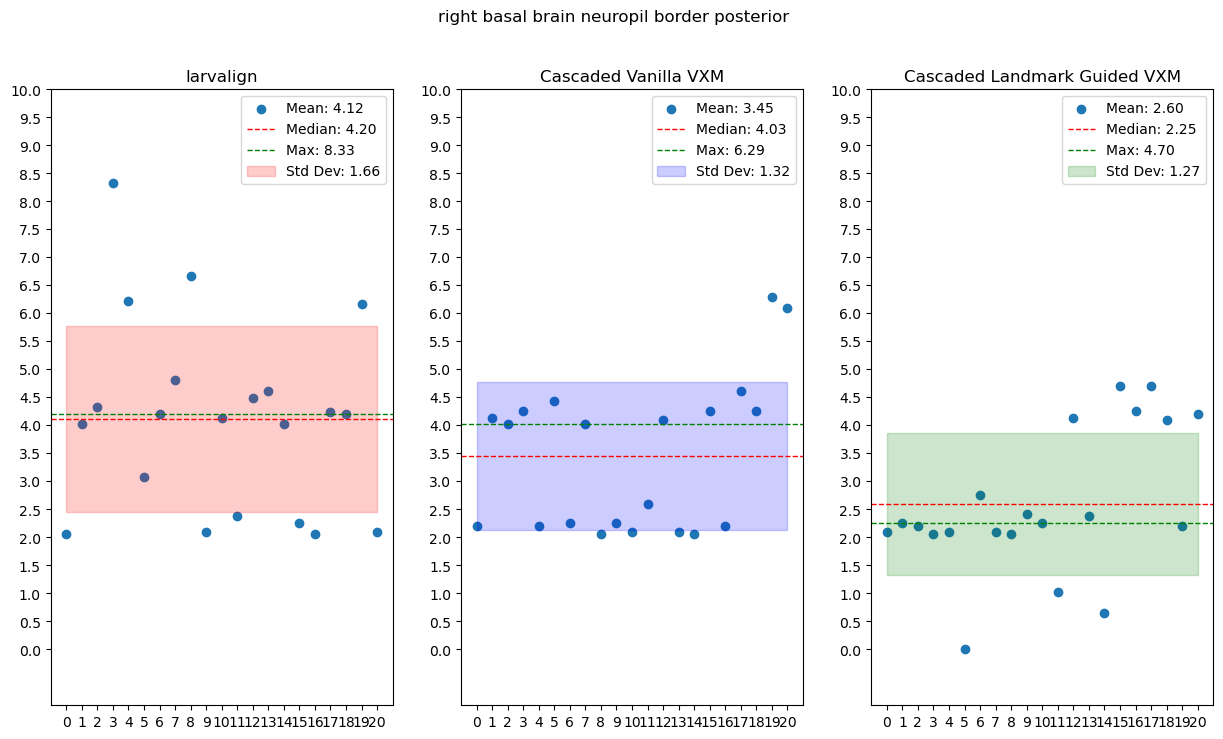
\includegraphics[width=0.75\columnwidth]{resources/chapter5_fresh/output/right basal brain neuropil border posterior.png}
		\caption{LRE plot distribution for "right basal brain neuropil border posterior" landmark point measured across different scans from the "medium" quality \texttt{Larvalign dataset}.}
		\label{fig:landmark4}
	\end{figure}

	\begin{figure}[h]
		\centering
		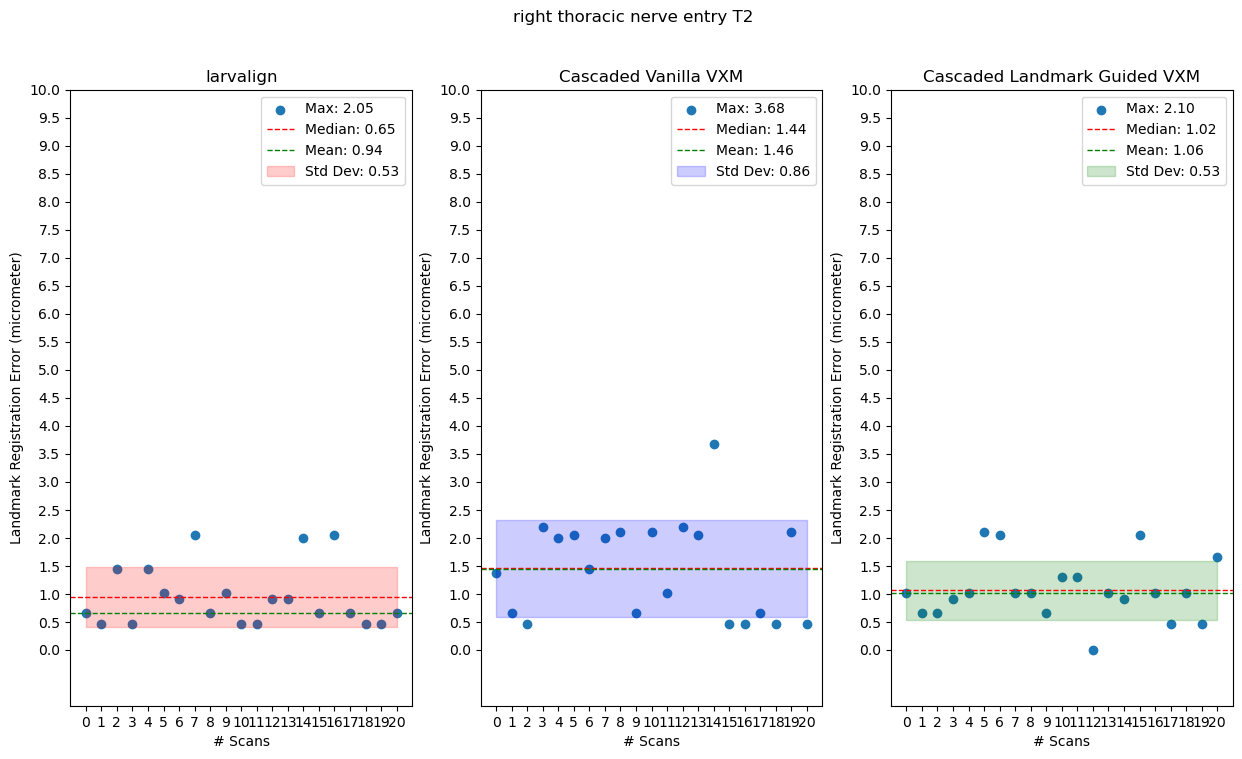
\includegraphics[width=0.75\columnwidth]{resources/chapter5_fresh/output/right thoracic nerve entry T2.png}
		\caption{LRE plot distribution for "right thoracic nerve entry T2" landmark point measured across different scans from the "medium" quality \texttt{Larvalign dataset}.}
		\label{fig:landmark5}
	\end{figure}

	\begin{figure}[h]
		\centering
		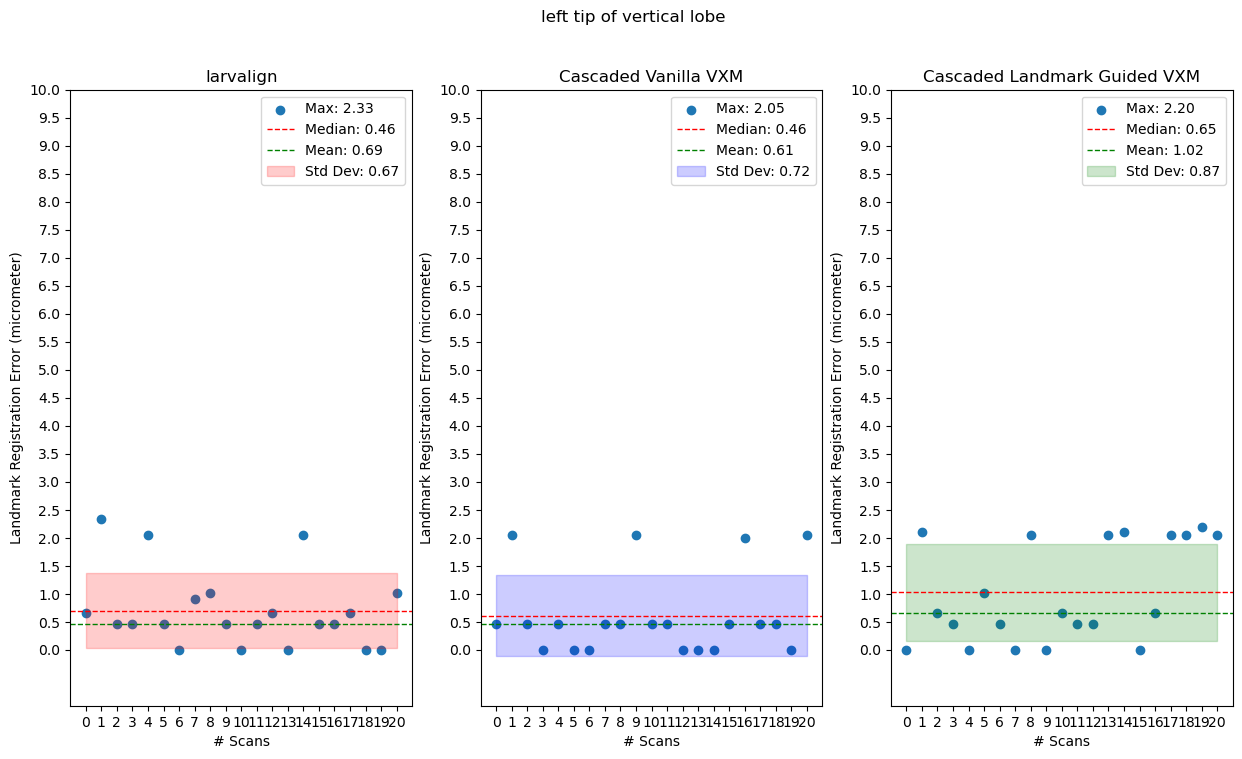
\includegraphics[width=0.75\columnwidth]{resources/chapter5_fresh/output/left tip of vertical lobe.png}
		\caption{LRE plot distribution for "left tip of vertical lobe" landmark point measured across different scans from the "medium" quality \texttt{Larvalign dataset}.}
		\label{fig:landmark6}
	\end{figure}

	\begin{figure}[h]
		\centering
		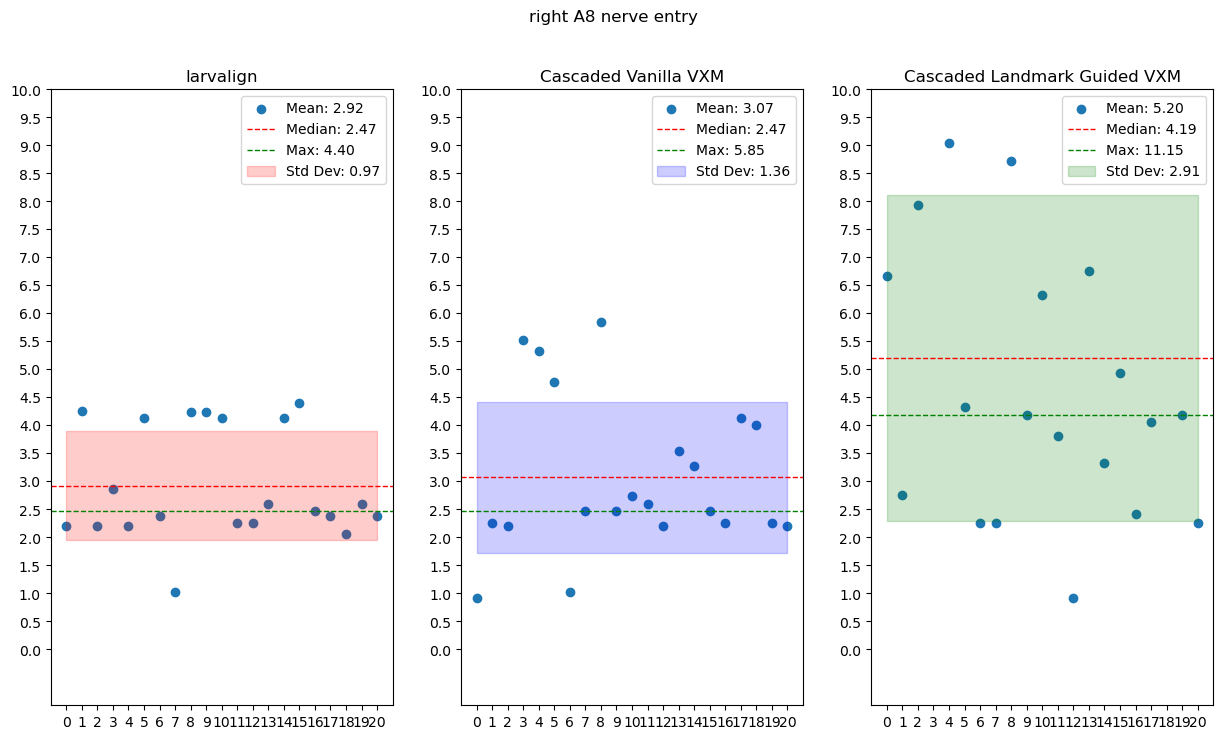
\includegraphics[width=0.75\columnwidth]{resources/chapter5_fresh/output/right A8 nerve entry.png}
		\caption{LRE plot distribution for "right A8 nerve entry" landmark point measured across different scans from the "medium" quality \texttt{Larvalign dataset}.}
		\label{fig:landmark7}
	\end{figure}

	\begin{figure}[h]
		\centering
		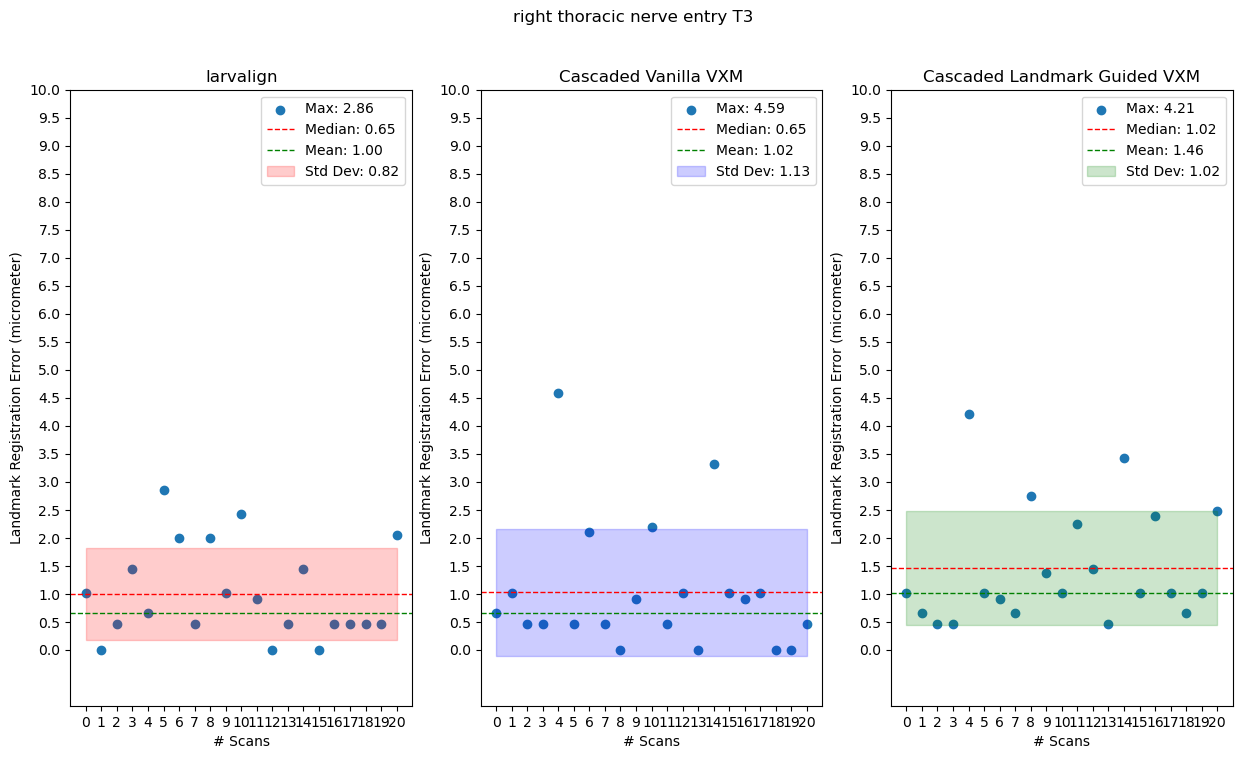
\includegraphics[width=0.75\columnwidth]{resources/chapter5_fresh/output/right thoracic nerve entry T3.png}
		\caption{LRE plot distribution for "right thoracic nerve entry T3" landmark point measured across different scans from the "medium" quality \texttt{Larvalign dataset}.}
		\label{fig:landmark8}
	\end{figure}

	\begin{figure}[h!]
		\centering
		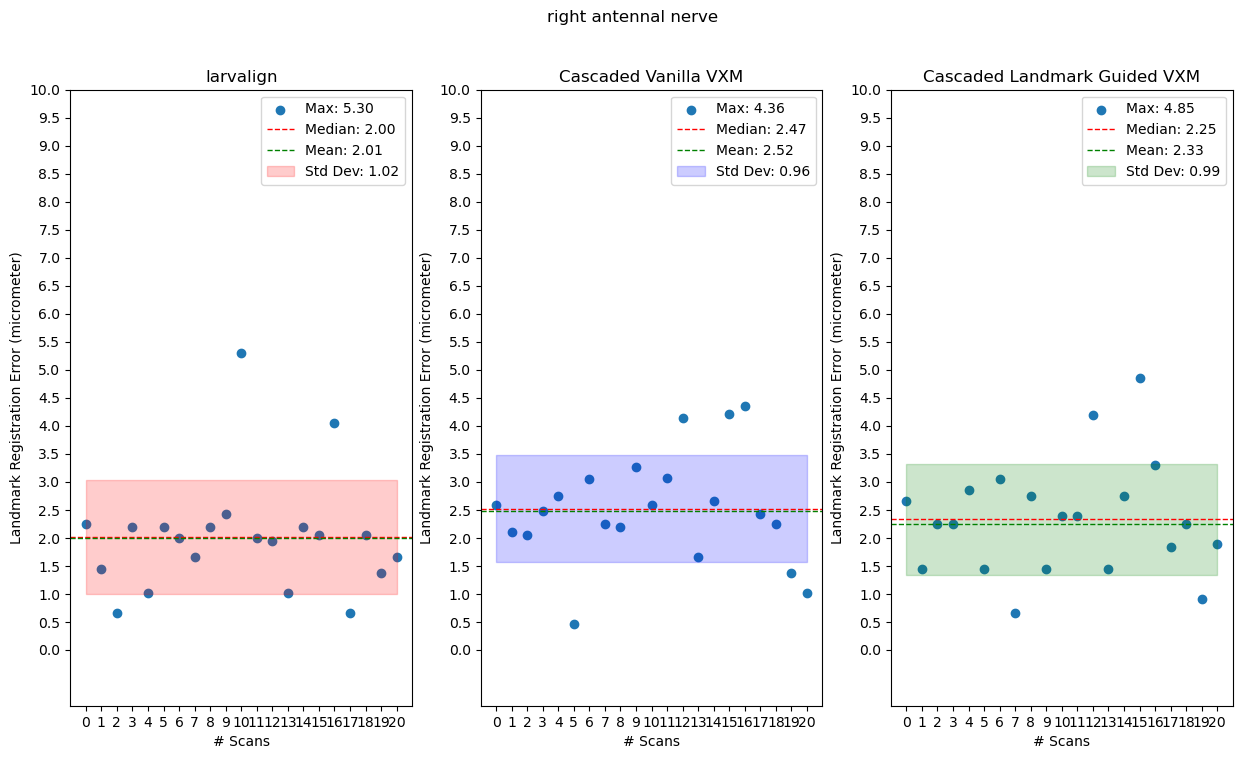
\includegraphics[width=0.75\columnwidth]{resources/chapter5_fresh/output/right antennal nerve.png}
		\caption{LRE plot distribution for "right antennal nerve" landmark point measured across different scans from the "medium" quality \texttt{Larvalign dataset}.}
		\label{fig:landmark9}
	\end{figure}

	\begin{figure}[h!]
		\centering
		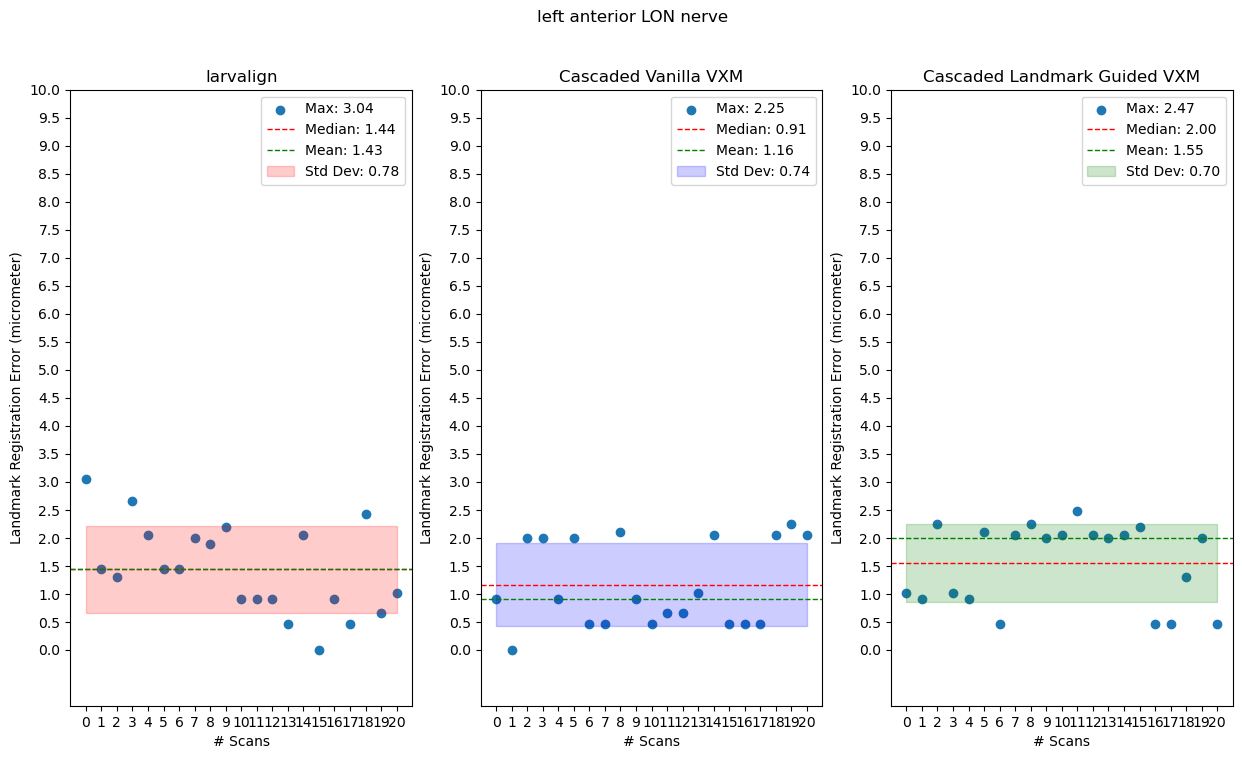
\includegraphics[width=0.75\columnwidth]{resources/chapter5_fresh/output/left anterior LON nerve.png}
		\caption{LRE plot distribution for "left anterior LON nerve" landmark point measured across different scans from the "medium" quality \texttt{Larvalign dataset}.}
		\label{fig:landmark10}
	\end{figure}

	\begin{figure}[h!]
		\centering
		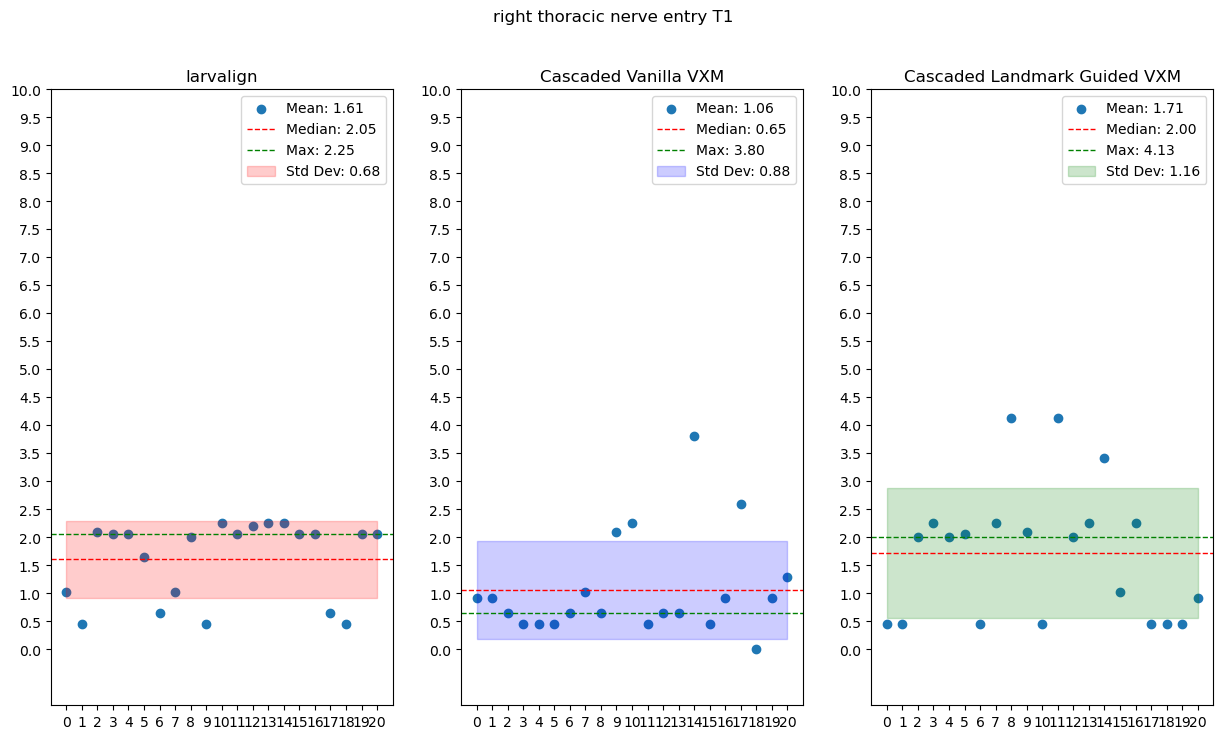
\includegraphics[width=0.75\columnwidth]{resources/chapter5_fresh/output/right thoracic nerve entry T1.png}
		\caption{LRE plot distribution for "right thoracic nerve entry T1" landmark point measured across different scans from the "medium" quality \texttt{Larvalign dataset}.}
		\label{fig:landmark11}
	\end{figure}

	\begin{figure}[h!]
		\centering
		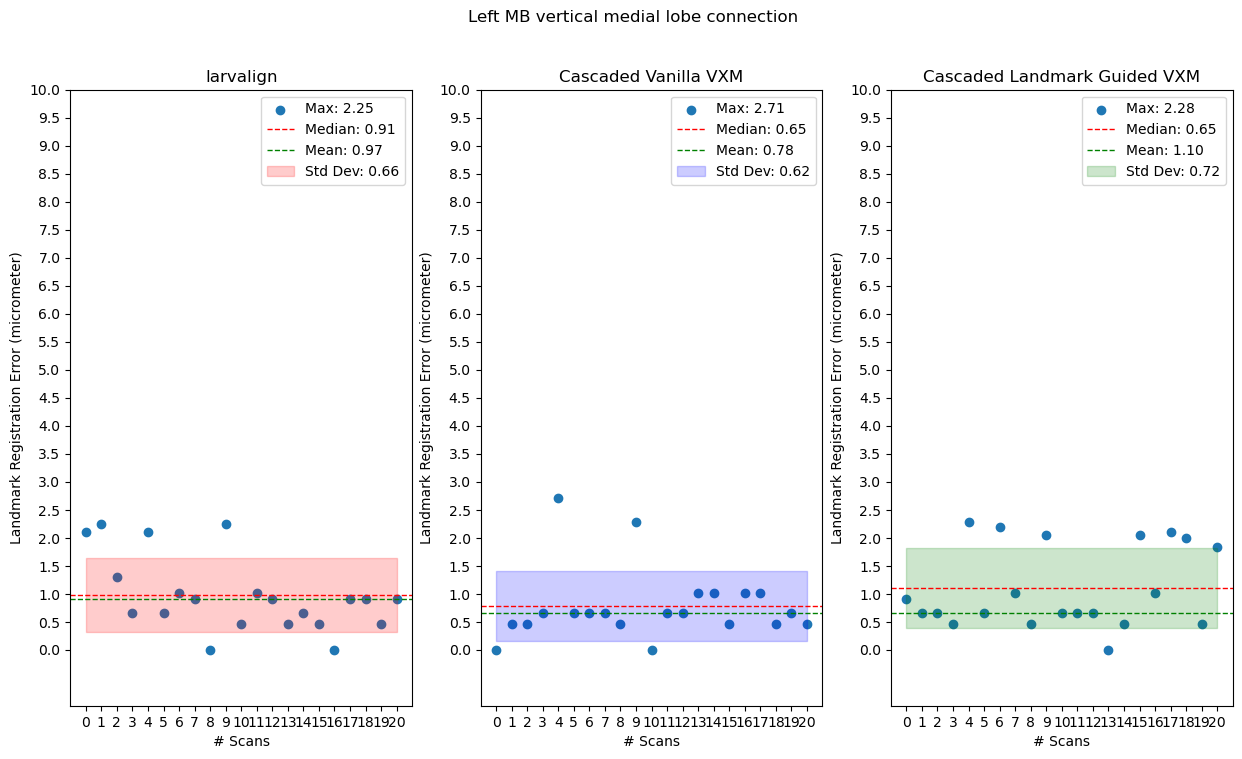
\includegraphics[width=0.75\columnwidth]{resources/chapter5_fresh/output/Left MB vertical medial lobe connection.png}
		\caption{LRE plot distribution for "Left MB vertical medial lobe connection" landmark point measured across different scans from the "medium" quality \texttt{Larvalign dataset}.}
		\label{fig:landmark12}
	\end{figure}

	\begin{figure}[h!]
		\centering
		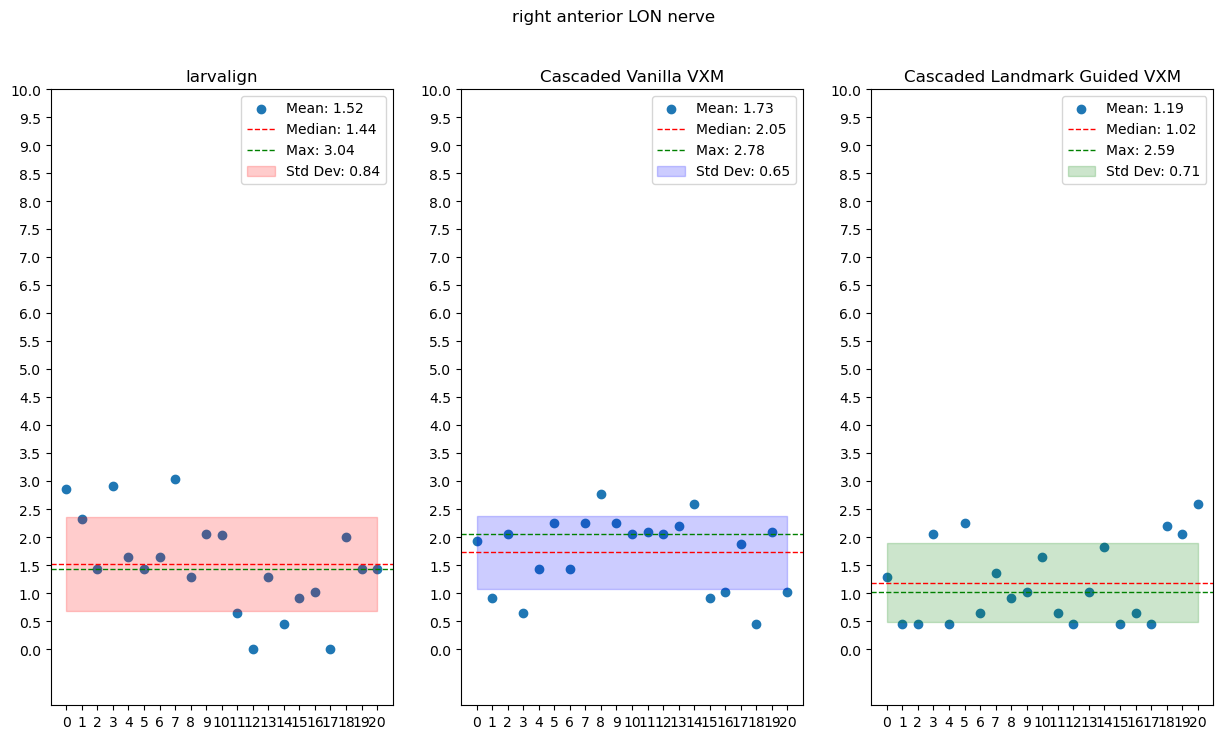
\includegraphics[width=0.75\columnwidth]{resources/chapter5_fresh/output/right anterior LON nerve.png}
		\caption{LRE plot distribution for "right anterior LON nerve" landmark point measured across different scans from the "medium" quality \texttt{Larvalign dataset}.}
		\label{fig:landmark13}
	\end{figure}

	\begin{figure}[h!]
		\centering
		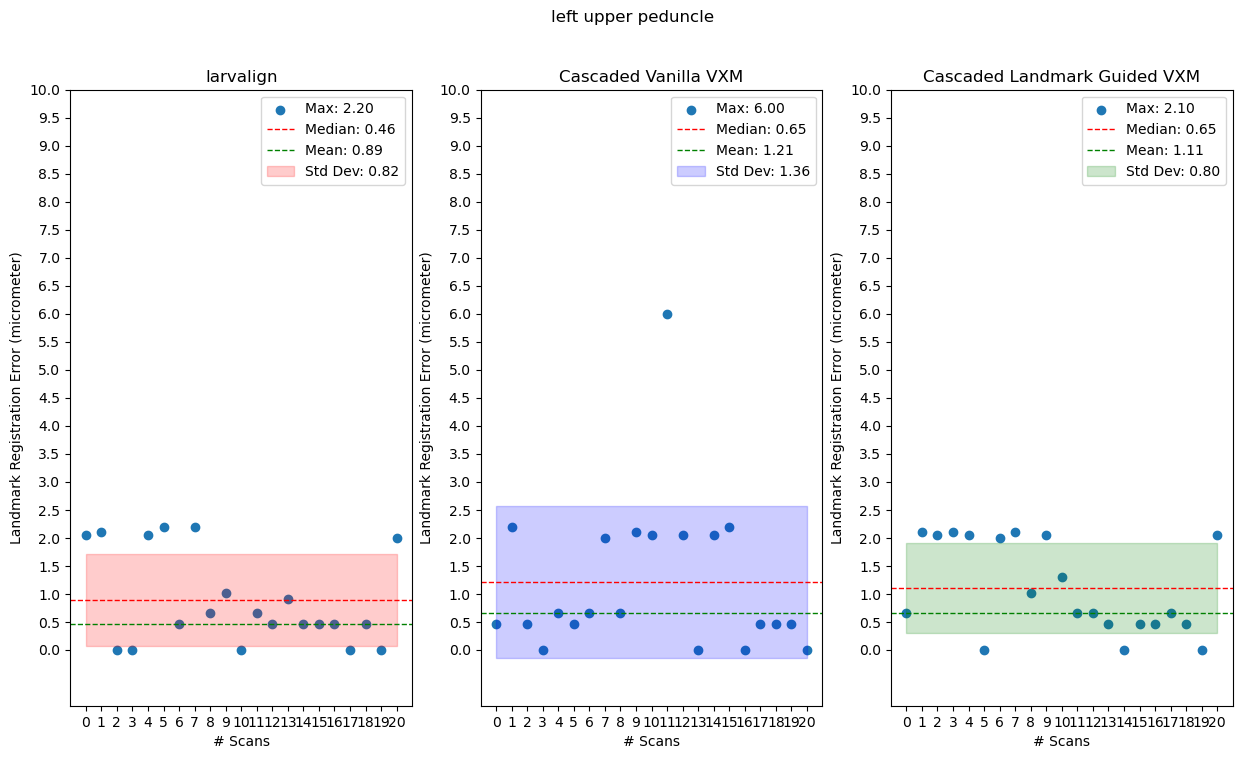
\includegraphics[width=0.75\columnwidth]{resources/chapter5_fresh/output/left upper peduncle.png}
		\caption{LRE plot distribution for "left upper peduncle" landmark point measured across different scans from the "medium" quality \texttt{Larvalign dataset}.}
		\label{fig:landmark14}
	\end{figure}

	\begin{figure}[h!]
		\centering
		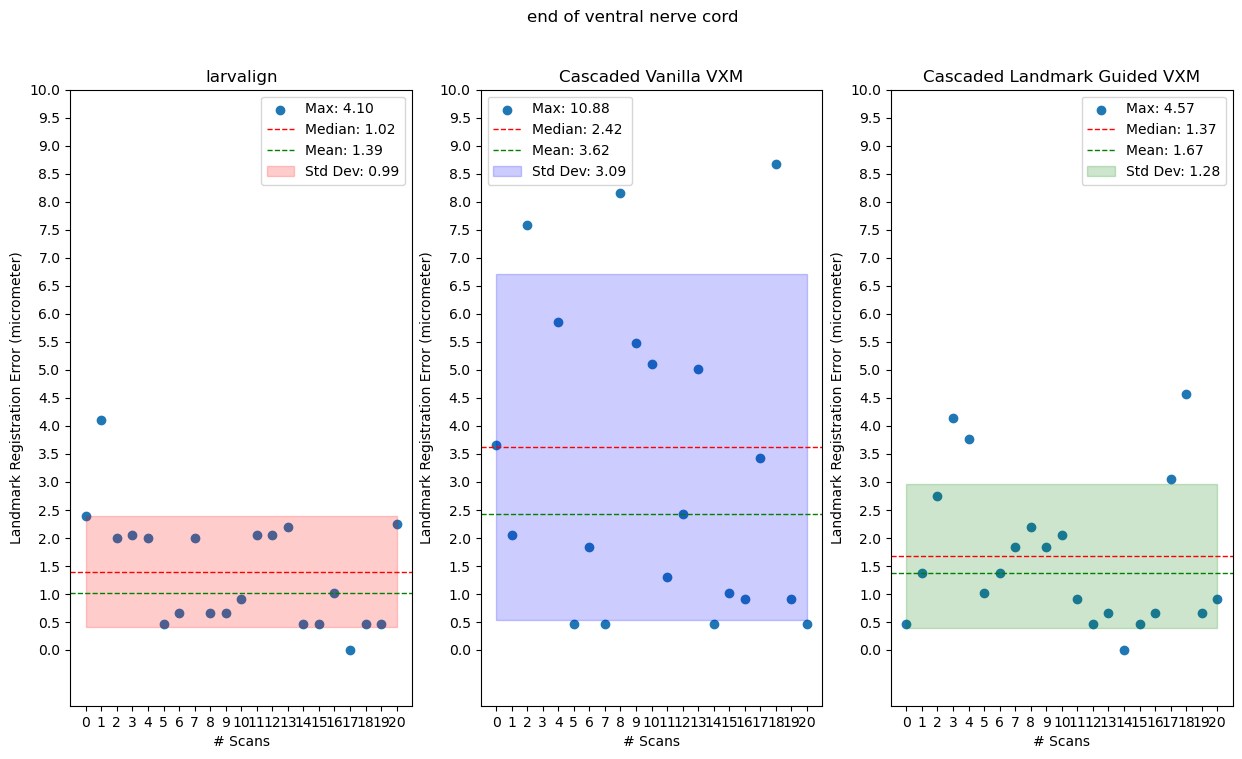
\includegraphics[width=0.75\columnwidth]{resources/chapter5_fresh/output/end of ventral nerve cord.png}
		\caption{LRE plot distribution for "end of ventral nerve cord" landmark point measured across different scans from the "medium" quality \texttt{Larvalign dataset}.}
		\label{fig:landmark15}
	\end{figure}

	\begin{figure}[h!]
		\centering
		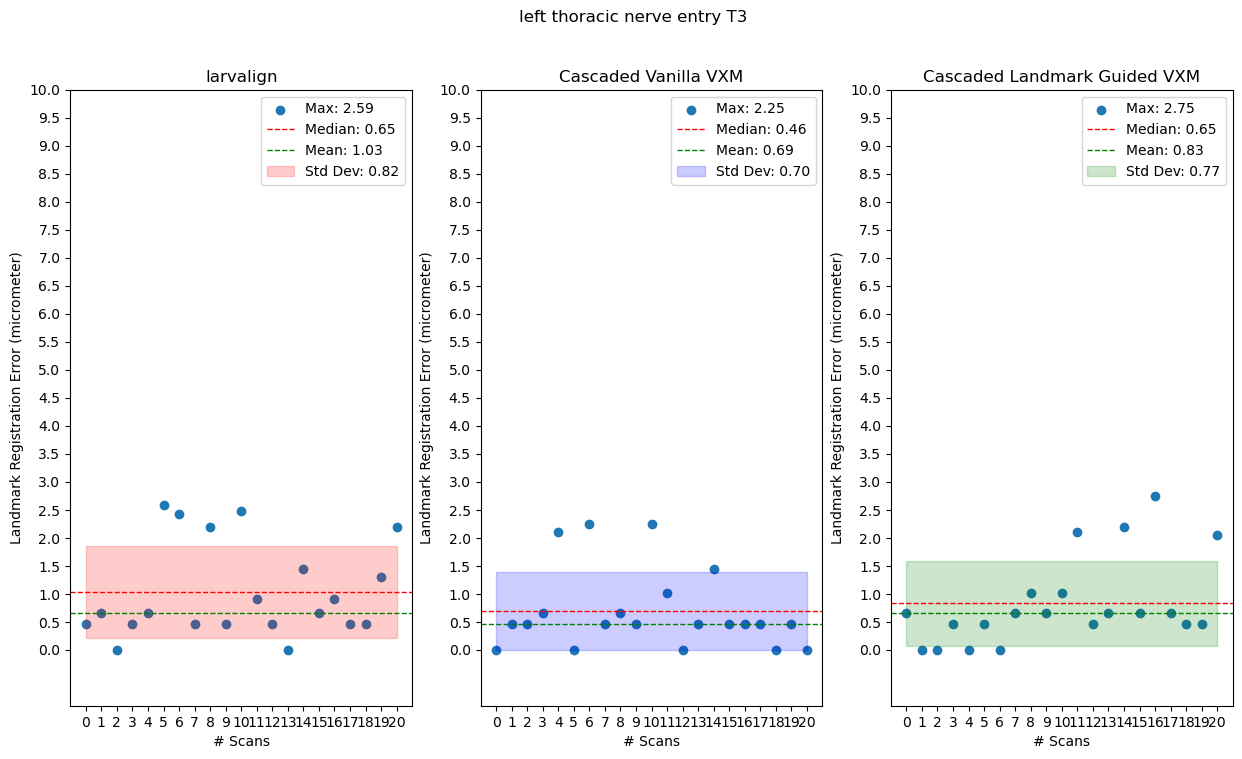
\includegraphics[width=0.75\columnwidth]{resources/chapter5_fresh/output/left thoracic nerve entry T3.png}
		\caption{LRE plot distribution for "left thoracic nerve entry T3" landmark point measured across different scans from the "medium" quality \texttt{Larvalign dataset}.}
		\label{fig:landmark16}
	\end{figure}

	\begin{figure}[h!]
		\centering
		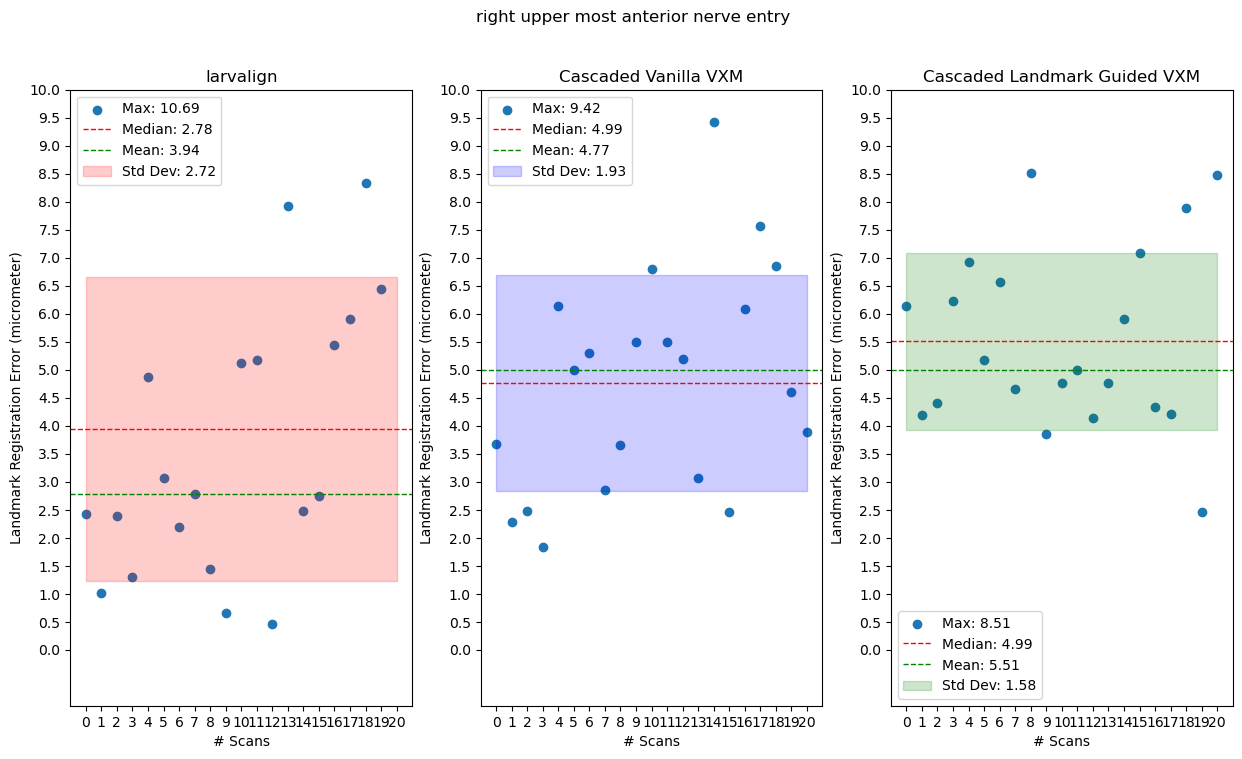
\includegraphics[width=0.75\columnwidth]{resources/chapter5_fresh/output/right upper most anterior nerve entry.png}
		\caption{LRE plot distribution for "right upper most anterior nerve entry" landmark point measured across different scans from the "medium" quality \texttt{Larvalign dataset}.}
		\label{fig:landmark17}
	\end{figure}

	\begin{figure}[h!]
		\centering
		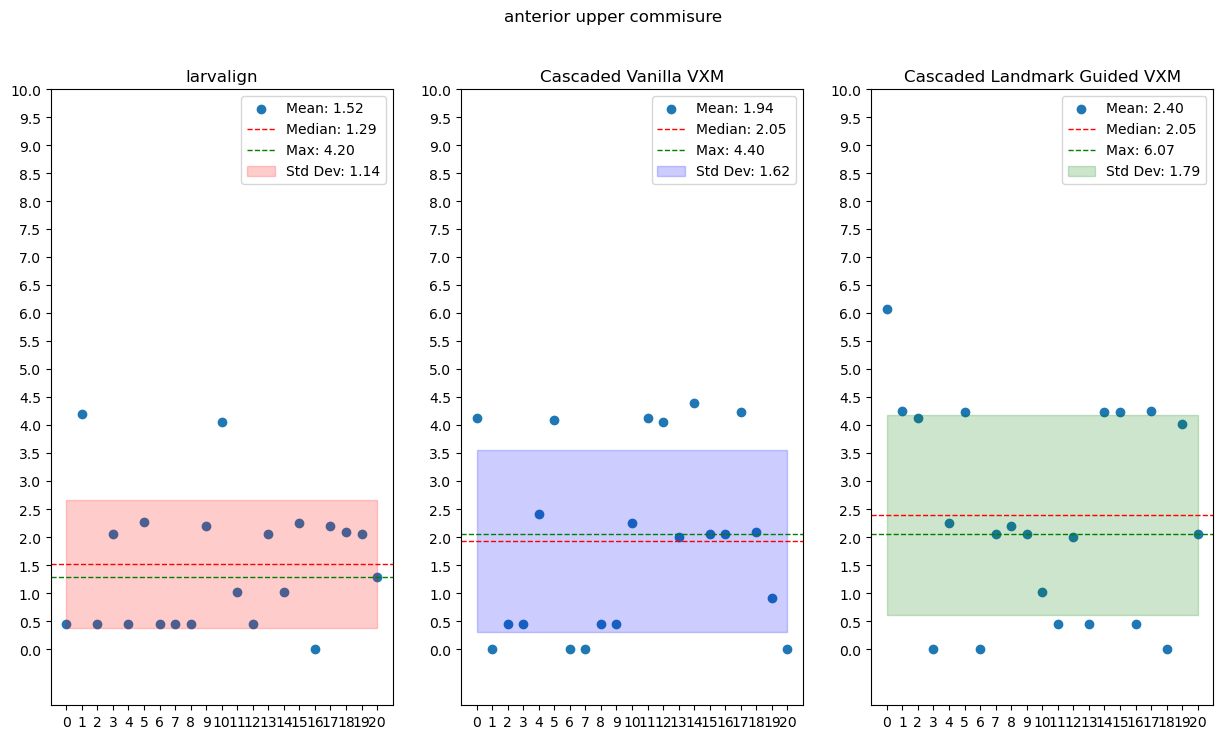
\includegraphics[width=0.75\columnwidth]{resources/chapter5_fresh/output/anterior upper commisure.png}
		\caption{LRE plot distribution for "anterior upper commisure" landmark point measured across different scans from the "medium" quality \texttt{Larvalign dataset}.}
		\label{fig:landmark18}
	\end{figure}

	\begin{figure}[h!]
		\centering
		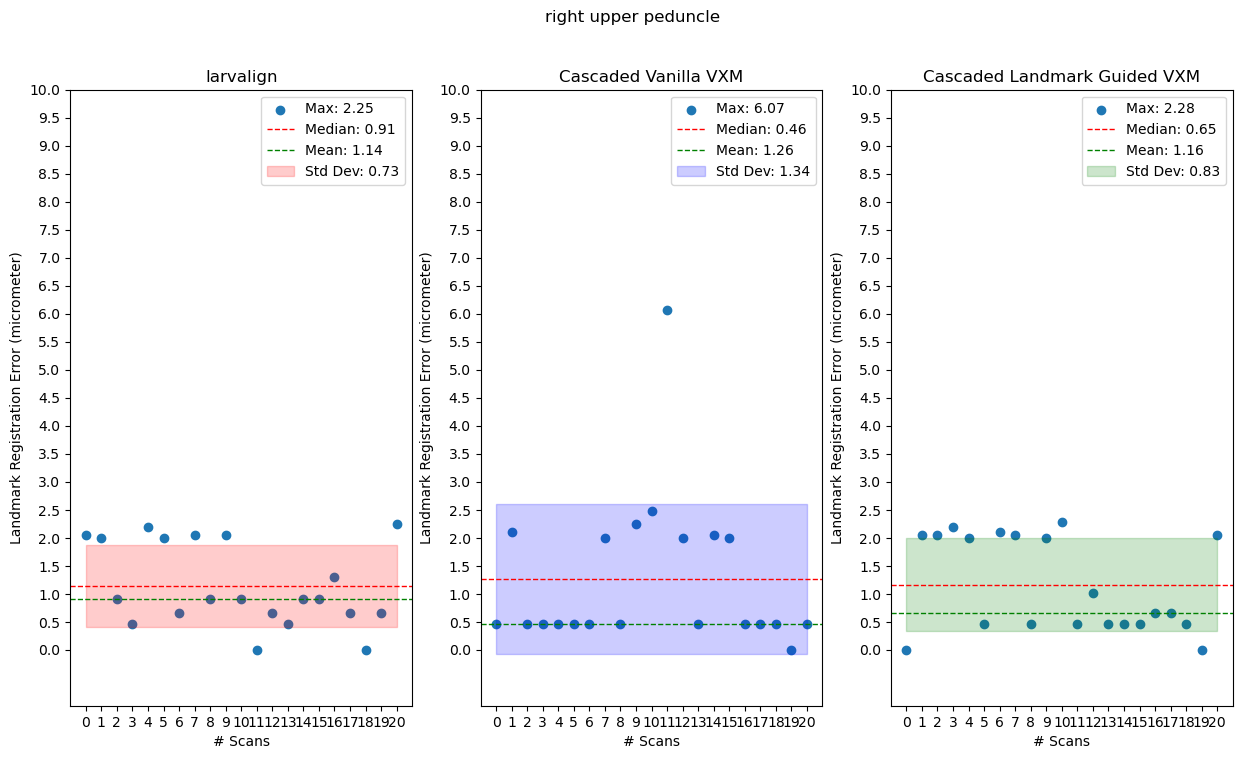
\includegraphics[width=0.75\columnwidth]{resources/chapter5_fresh/output/right upper peduncle.png}
		\caption{LRE plot distribution for "right upper peduncle" landmark point measured across different scans from the "medium" quality \texttt{Larvalign dataset}.}
		\label{fig:landmark19}
	\end{figure}

	\begin{figure}[h!]
		\centering
		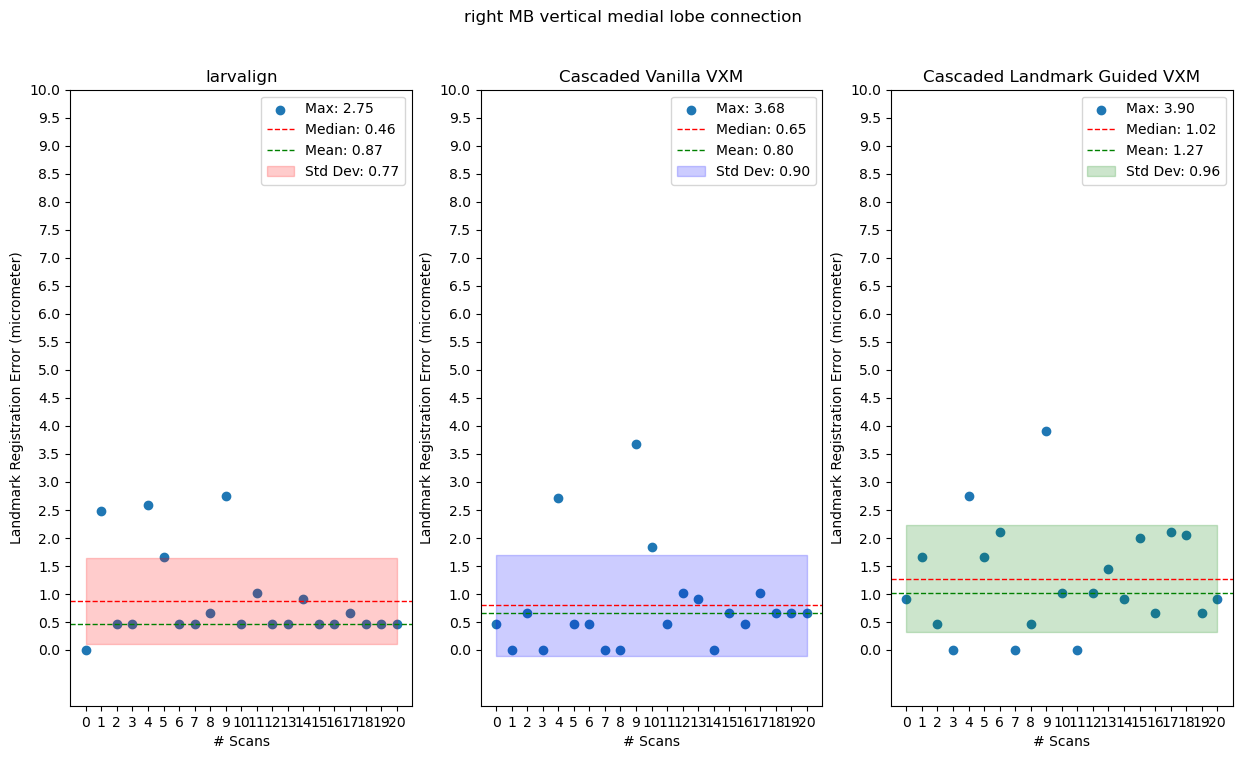
\includegraphics[width=0.75\columnwidth]{resources/chapter5_fresh/output/right MB vertical medial lobe connection.png}
		\caption{LRE plot distribution for "right MB vertical medial lobe connection" landmark point measured across different scans from the "medium" quality \texttt{Larvalign dataset}.}
		\label{fig:landmark20}
	\end{figure}

	\begin{figure}[h!]
		\centering
		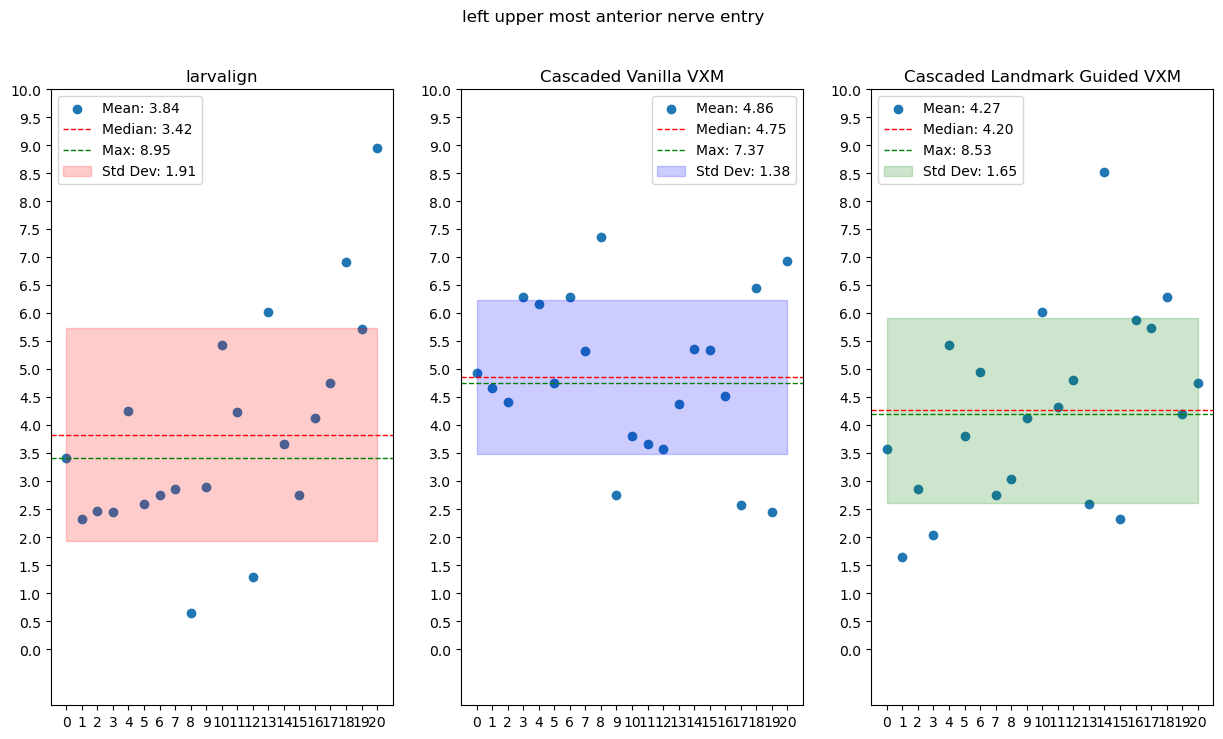
\includegraphics[width=0.75\columnwidth]{resources/chapter5_fresh/output/left upper most anterior nerve entry.png}
		\caption{LRE plot distribution for "left upper most anterior nerve entry" landmark point measured across different scans from the "medium" quality \texttt{Larvalign dataset}.}
		\label{fig:landmark21}
	\end{figure}

	\begin{figure}[h!]
		\centering
		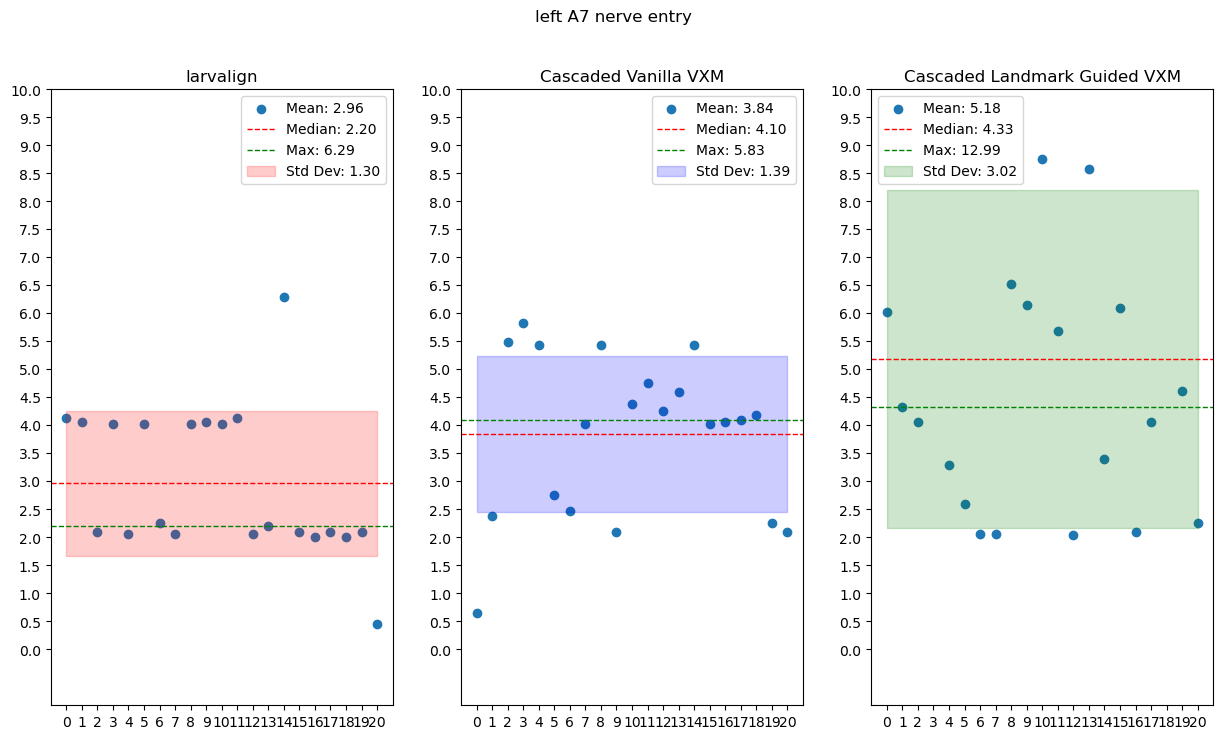
\includegraphics[width=0.75\columnwidth]{resources/chapter5_fresh/output/left A7 nerve entry.png}
		\caption{LRE plot distribution for "left A7 nerve entry" landmark point measured across different scans from the "medium" quality \texttt{Larvalign dataset}.}
		\label{fig:landmark22}
	\end{figure}

	\begin{figure}[h!]
		\centering
		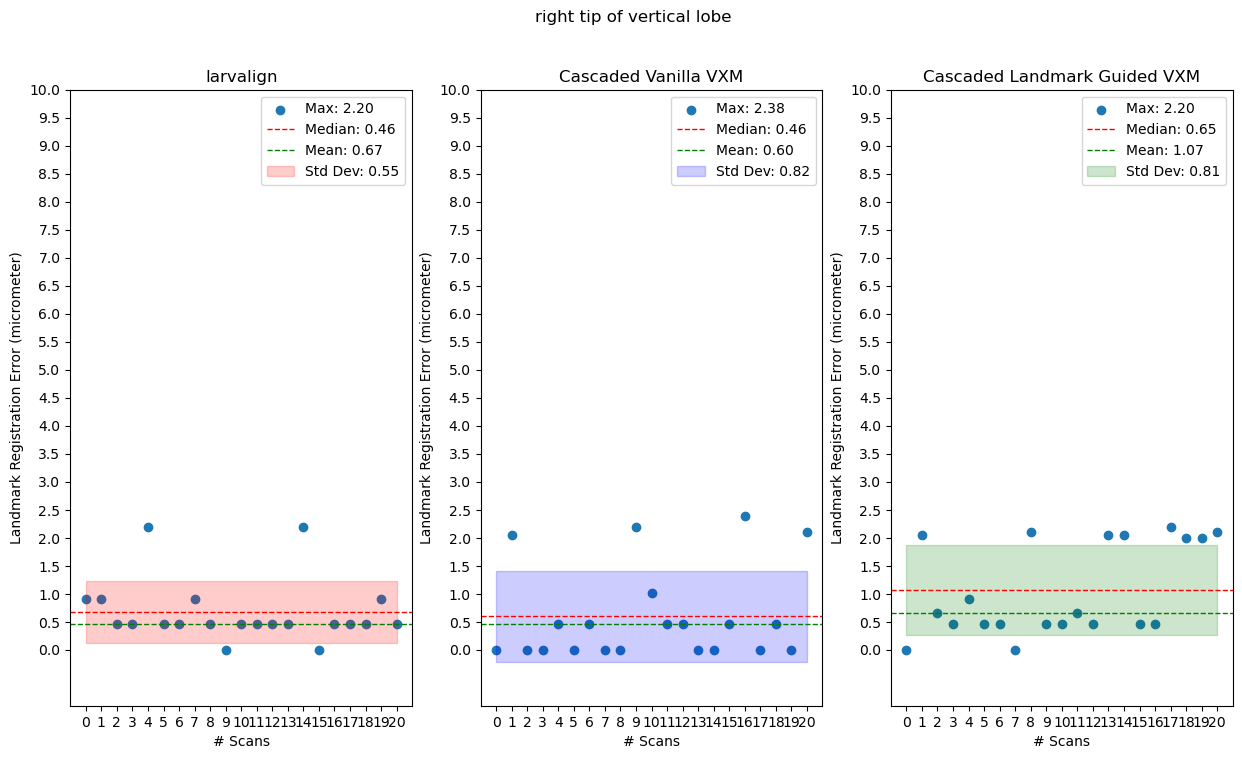
\includegraphics[width=0.75\columnwidth]{resources/chapter5_fresh/output/right tip of vertical lobe.png}
		\caption{LRE plot distribution for "right tip of vertical lobe" landmark point measured across different scans from the "medium" quality \texttt{Larvalign dataset}.}
		\label{fig:landmark23}
	\end{figure}

	\begin{figure}[h!]
		\centering
		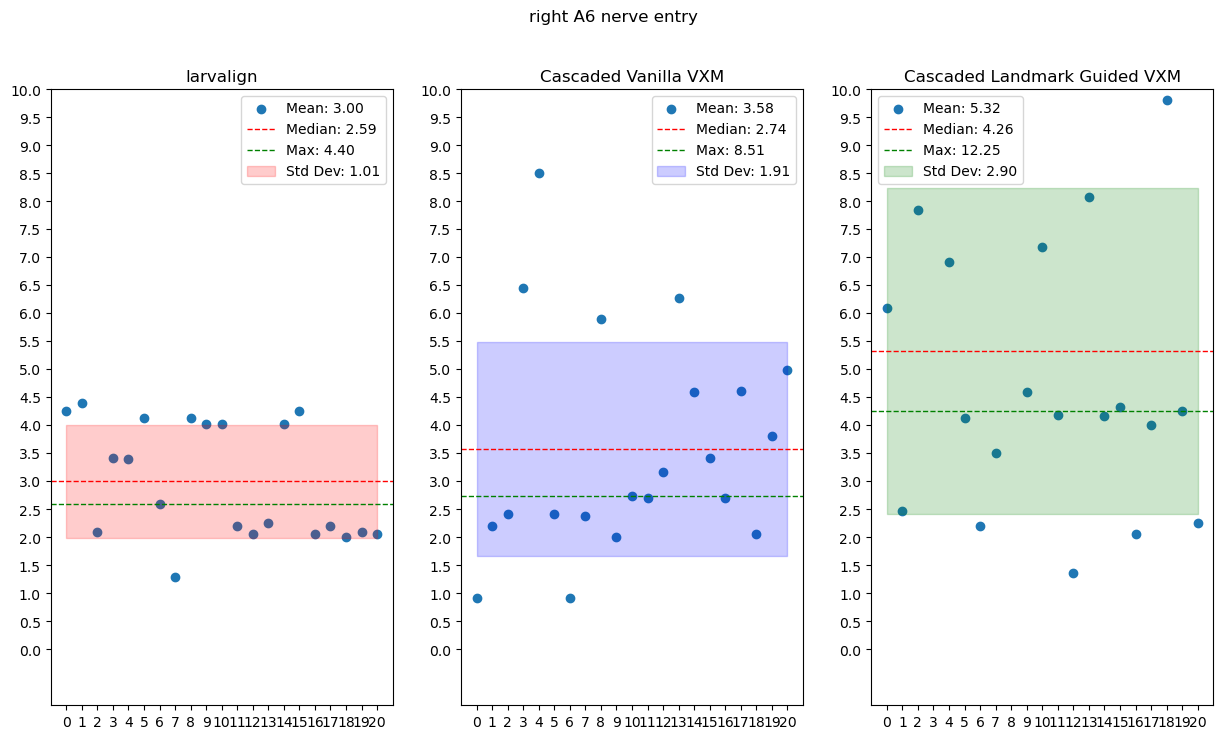
\includegraphics[width=0.75\columnwidth]{resources/chapter5_fresh/output/right A6 nerve entry.png}
		\caption{LRE plot distribution for "right A6 nerve entry" landmark point measured across different scans from the "medium" quality \texttt{Larvalign dataset}.}
		\label{fig:landmark24}
	\end{figure}

	\begin{figure}[h!]
		\centering
		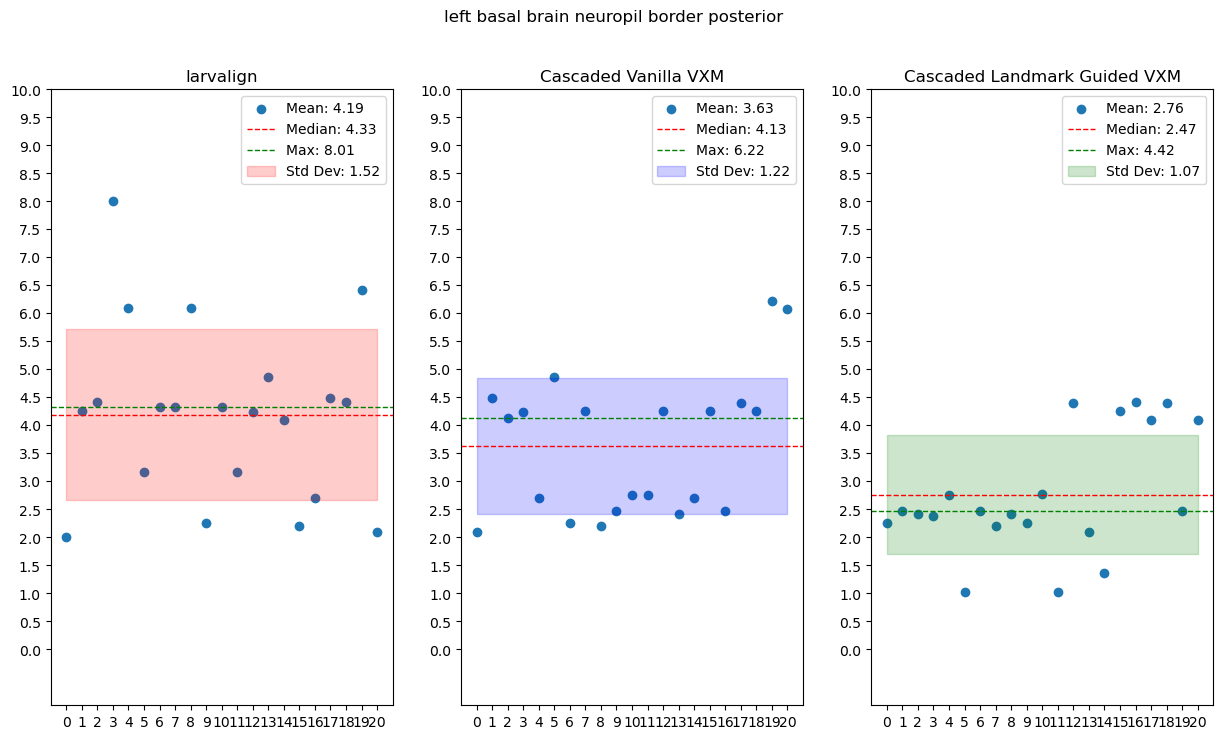
\includegraphics[width=0.75\columnwidth]{resources/chapter5_fresh/output/left basal brain neuropil border posterior.png}
		\caption{LRE plot distribution for "left basal brain neuropil border posterior" landmark point measured across different scans from the "medium" quality \texttt{Larvalign dataset}.}
		\label{fig:landmark25}
	\end{figure}

	\begin{figure}[h!]
		\centering
		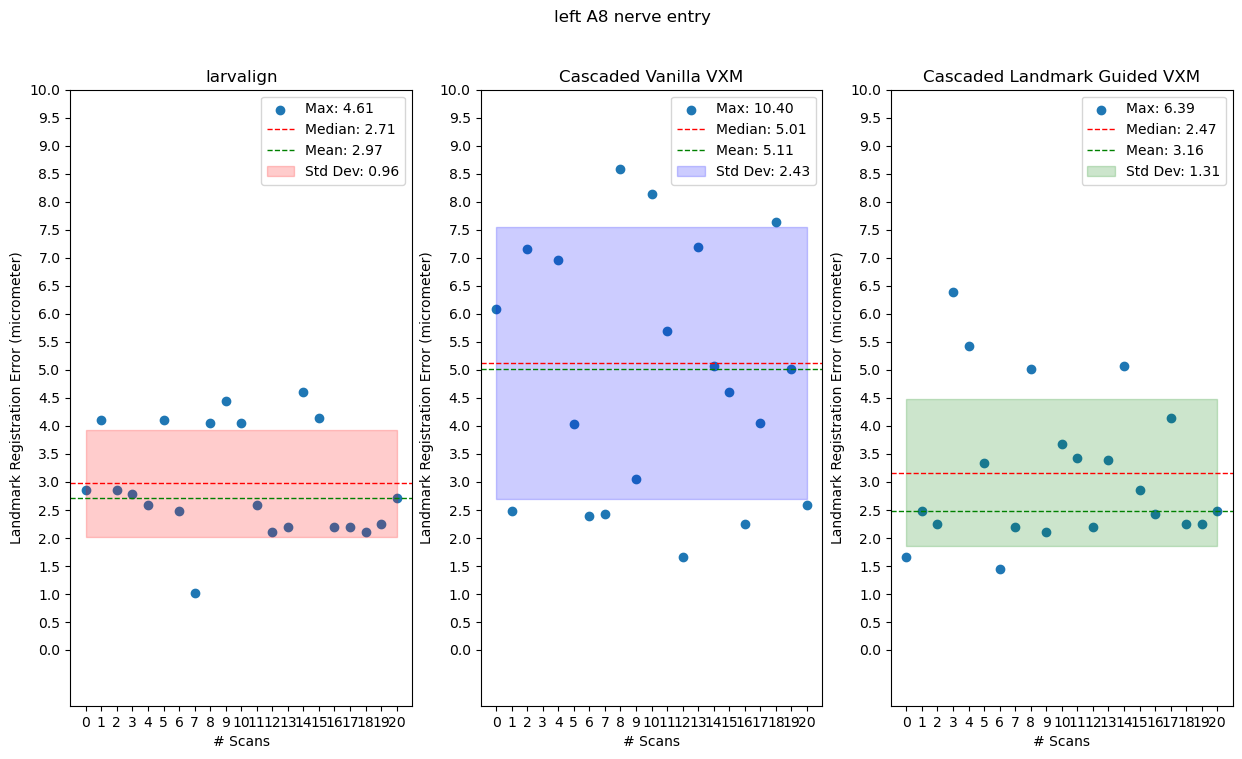
\includegraphics[width=0.75\columnwidth]{resources/chapter5_fresh/output/left A8 nerve entry.png}
		\caption{LRE plot distribution for "left A8 nerve entry" landmark point measured across different scans from the "medium" quality \texttt{Larvalign dataset}.}
		\label{fig:landmark26}
	\end{figure}

	\begin{figure}[h!]
		\centering
		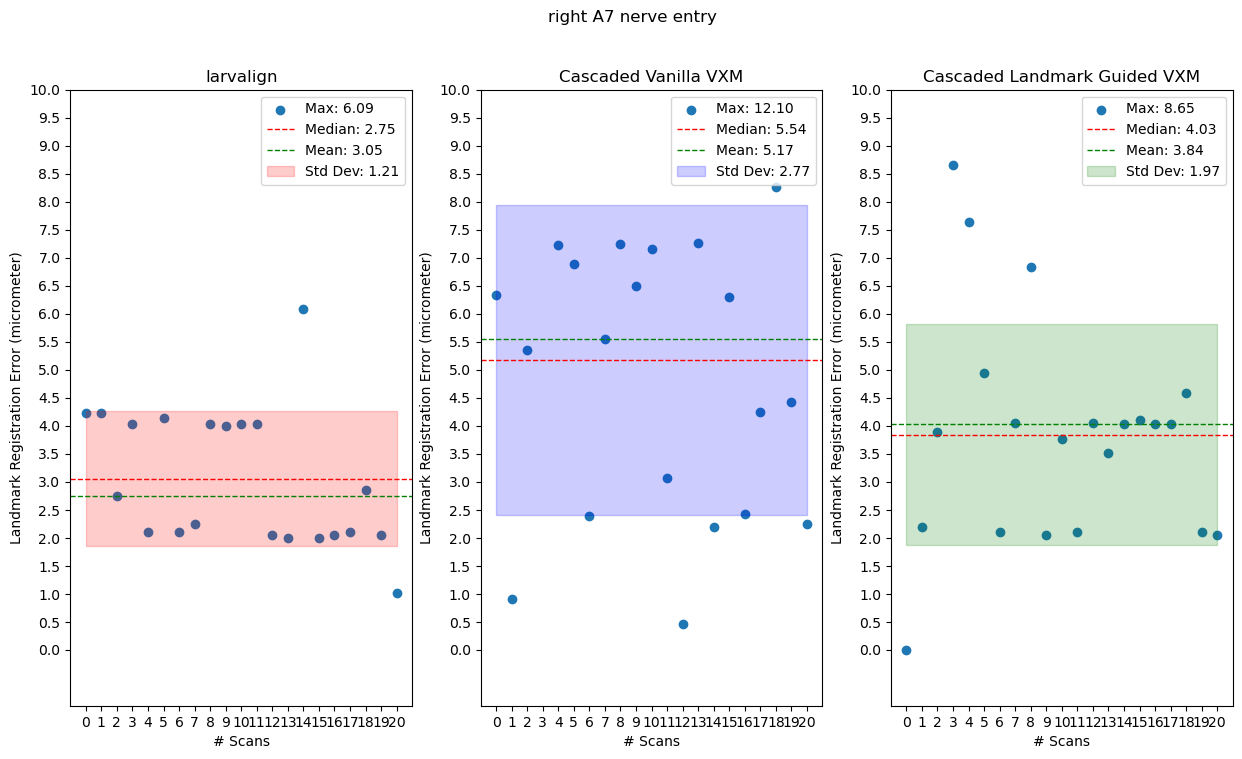
\includegraphics[width=0.75\columnwidth]{resources/chapter5_fresh/output/right A7 nerve entry.png}
		\caption{LRE plot distribution for "right A7 nerve entry" landmark point measured across different scans from the "medium" quality \texttt{Larvalign dataset}.}
		\label{fig:landmark27}
	\end{figure}

	\begin{figure}[h!]
		\centering
		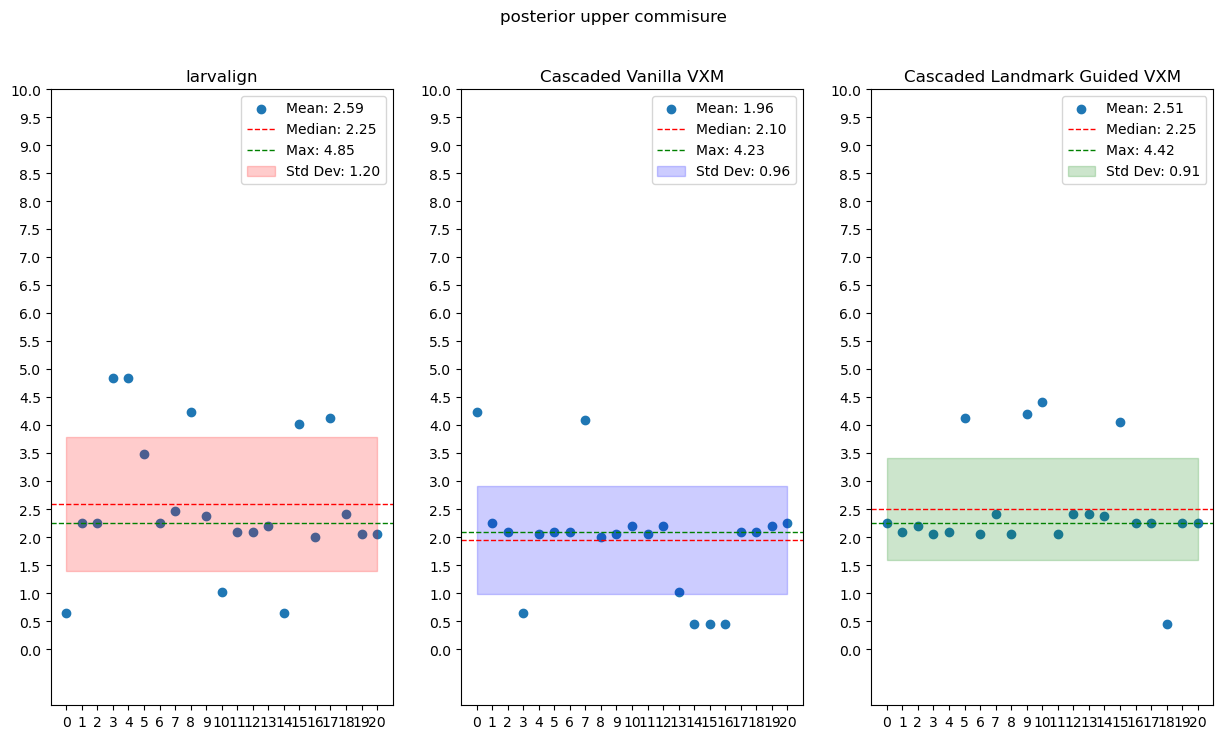
\includegraphics[width=0.75\columnwidth]{resources/chapter5_fresh/output/posterior upper commisure.png}
		\caption{LRE plot distribution for "posterior upper commisure" landmark point measured across different scans from the "medium" quality \texttt{Larvalign dataset}.}
		\label{fig:landmark28}
	\end{figure}

	\begin{figure}[h!]
		\centering
		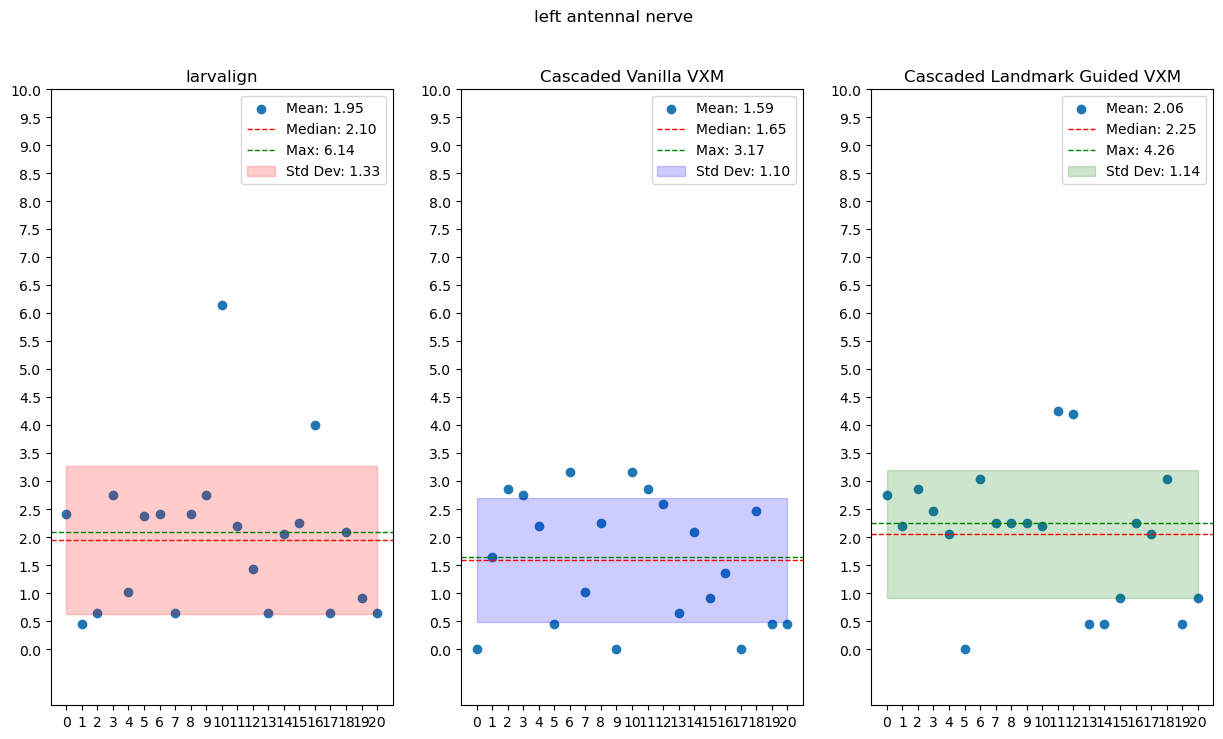
\includegraphics[width=0.75\columnwidth]{resources/chapter5_fresh/output/left antennal nerve.png}
		\caption{LRE plot distribution for "left antennal nerve" landmark point measured across different scans from the "medium" quality \texttt{Larvalign dataset}.}
		\label{fig:landmark29}
	\end{figure}

	\begin{figure}[h!]
		\centering
		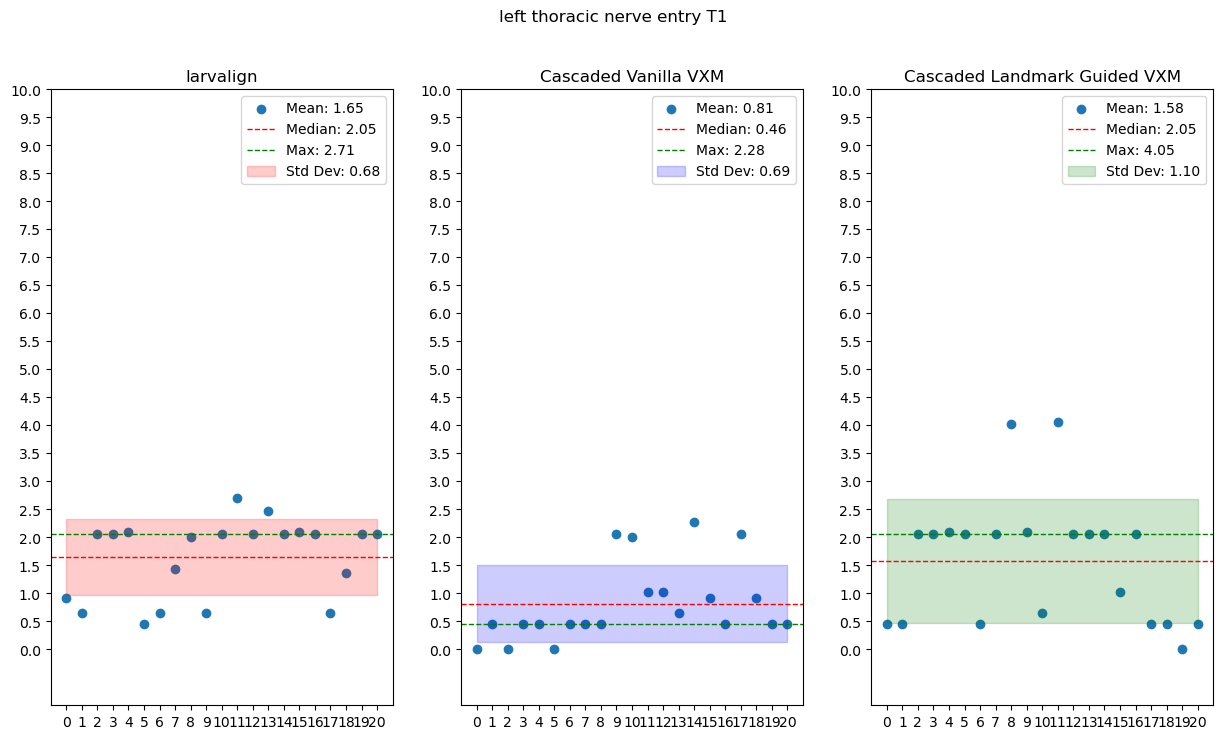
\includegraphics[width=0.75\columnwidth]{resources/chapter5_fresh/output/left thoracic nerve entry T1.png}
		\caption{LRE plot distribution for "left thoracic nerve entry T1" landmark point measured across different scans from the "medium" quality \texttt{Larvalign dataset}.}
		\label{fig:landmark30}
	\end{figure}

